\section{Telemetry}

\subsection{Overview}
\label{sec:bg_telemetry_overview}

The Formula SAE 2010 vehicle utilizes several sensors for monitoring key elements of the engine and drivetrain. As mentioned previously in Sec. \ref{sec:ECU}, the ECU uses these sensor readings to adjust the fuel injector and spark coil timings. However, the data gathered from these sensors can be very useful to determining the overall performance and health of the vehicle. 

Longitudinal and strain data are also important, as they can be used to track driver performance and to prevent mechanical fatigue and failure. Several sensors have been introduced in previous years to accomplish this, but the ECU makes no provisions for handling data that is not engine-related. A secondary device known as the \emph{Data Acquisition Device} (DAC) was introduced to record and broadcast secondary sensor data.

Both the ECU and the DAC interface with proprietary software over hard-wired serial links. It was recognized in previous years that a wireless serial link would be required to gather data in real-time while the vehicle was actually performing in the field. Several solutions were proposed and introduced, but none of them have performed satisfactorily.

\subsection{Sensors}

The engine has a set of sensors attached to it that aide the ECU in determining the best parameters for controlling the fuel injection and spark coil timings. These include:

\begin{itemize}

\item The \emph{oxygen} sensor, which monitors the amount of oxygen present in the exhaust of the engine. This information, when coupled with other sensor information, can be used to calculate the air-fuel mixture ratio being combusted \cite{o2sensor}.

\item The \emph{Manifold Absolute Pressure} (MAP) sensor, which monitors the pressure in the manifold. The ECU uses this information to calculate the mass flow rate of air in the engine, which is also used to adjust the air-fuel mixture ratio being combusted \cite{mapsensor}.

\item The \emph{oil pressure} sensor, which is used to ensure enough oil pressure is present to keep the moving metal parts inside the engine are well-lubricated. A lack of oil pressure can cause an engine to \emph{seize}, meaning two moving parts in proximity have become stuck due to a lack of lubrication. This condition is typically fatal for an engine.

\item The \emph{water temperature} sensor, for monitoring the temperature of the coolant running through the engine block. The engine can become damaged if it is not adequately cooled, and an overheating engine can indicate to the crew that the coolant level is too low or there is a problem with the water pump.

\item The \emph{throttle position} sensor, to report the amount of throttle being applied by the driver, which in turn determines how much power is being demanded of the engine. This can be correlated with engine RPM data to determine how well the engine is responding to driver demands.

\item The \emph{cam position} sensor, which determines where the first cylinder is located in relation to it's combustion cycle. This data is used to determine when to inject each cylinder with fuel to maximize power output.

\item The \emph{crank position} sensor, for determining the rotational speed of the crankshaft, which therefore measures the actual engine RPM. 

\end{itemize}

Motional and strain data are also important and require logging and analysis. Sensors to capture these data include:

\begin{itemize}

\item A \emph{Global Positioning System} (GPS), which is used to track the absolute geographic position of the vehicle. 

\item \emph{Accelerometers} and \emph{ground speed detectors}, that are attached to the vehicle to determine it's acceleration and ground speed. Coupled with the GPS data, this can be used to measure driver performance and determine the best route to take through corners while on the track.

\item \emph{Strain gauges}, which are are attached to various members on the suspension and frame to determine the forces and strain the vehicle endures. These can be used to forecast fatigue and possible mechanical failure. 

\end{itemize}

\subsection{Data Acquisition Device}

The \emph{Data Acquisition Device} (DAC) is required to convert the locational and strain sensor data into digital signals that can be transmitted  the DAC used is the model DL1 from Race Technology \cite{DL1Dsheet}, as seen in Fig. \ref{fig:dl1_product}. The DL1 is an expandable data logger with built-in \unit{20}{\hertz} GPS and 3-axis accelerometer. 

Race Technology provides a software suite that communicates with the DAC using a documented serial protocol. Everything the DAC logs is output over it's serial channel in real-time.

\begin{figure}[H]
	\centering
		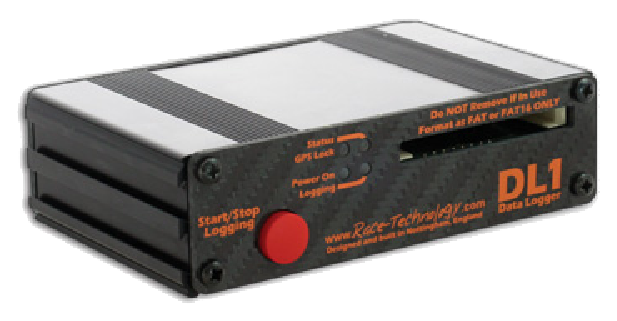
\includegraphics[scale=0.5]{background/figures/dl1.eps}
	\caption{The Race Systems DL1 data acquisition device.}
	\label{fig:dl1_product}
\end{figure}

\subsection{Cellular Link}

The 2005/2006 Formula team attempted to solve the wireless telemetry issue by using a CDMA-type cellular data link to broadcast ECU information to the pit crew. The team used a CDMA 1xRTT digital cellular network modem and a Soekris Engineering Linux-based microcomputer to interface between the ECU and cellular modem. The principle of operation was to broadcast ECU data through the modem to a local cell phone tower. The data would then be carried through the network, routed back to the local tower, and received by a modem connected to a laptop in the pit \cite{G26FinalRepo}.

This scheme created three very prominent disadvantages:

\begin{itemize}

\item Expensive wireless data and roaming charges were incurred while the team competed in the United States. 

\item There was a massive amount of lag introduced as the data travelled through the American and Candian cellular networks only to be received a few hundred metres away from the vehicle.

\item Only one device (the ECU) was able to be monitored in real-time. DAC data had to be logged on the device itself and downloaded later.

\end{itemize}

\subsection{Point-to-Point XBee Link}

From 2007 onward, the Formula team utilized a pair of off-the-shelf XBee Pro modems to wirelessly transmit information from the ECU to the pit crew. The XBee Pro modems estabilshed a transparent wireless link between the ECU and a pit-crew laptop. The ECU serial cable was plugged into a serial port located on a modem attached to the vehicle. An external antenna was run from the vehicle modem to the highest point of elevation on the vehicle, above the driver. The modem's twin was located in the pit, and attached to the pit crew laptop over another serial cable.

This scheme eliminated the need for a costly cellular solution and reduced transport lag, but was still far from optimal:

\begin{itemize}

\item Extensive interference was encountered, as similar modems on other competitor's vehicles were broadcasting on the same channel. When operating in "plug-and-play" mode, the broadcast channel must be adjusted manually on the device itself. Changing channels while in middle of a race is impossible, as it would require stopping the vehicle and exiting it.

\item As before, only the ECU data was being broadcast. To broadcast both ECU and DAC data would require two modems, which was not only cost prohibitive but also introduces more opportunity for interference. 

\end{itemize}
